%--------------------------------------------------------------------------------------------------
%
\chapter{Experiments}\label{chap:experiments}
%--------------------------------------------------------------------------------------------------

This chapter presents several experiments that explore how the theory relates
to practice. The first set of experiments focuses on global optimality
and convergence rates on synthetic data. We then move to
cross-lingual document analysis and examine the performance
of our approach on the task of information retrieval based
on training sets with missing data. Finally we evaluate our
approach to cross-lingual cluster linking.

\section{Synthetic Experiments}\label{chap:experiments:synthetic}
We generated several multiview problem instances by varying the number
of views and number of dimensions per view in order to
compare the performance of local search methods and the proposed
SDP relaxation. The goal of these experiments was to see
under which conditions and how often do the global bounds
provide useful information. The main observations are that the
set of problems where the bounds are useful has a non-zero
measure and that the difficulty of the optimization problem
increases with the number of views and decreases with the
number of dimensions per view.

\subsection{Generating Synthetic Problem Instances}

Let $m$ denote the number of views (sets of variables) and
$n_i$ denote the dimensionality of $i$-th
view and $N := \sum_i n_i$. In all cases, we used the same number
of dimensions per view ($n_1 = n_2 = \cdots = n_m$). We used
three different methods to generate random correlation matrices.

The first method, the \textbf{random Gram matrix} method (see
\cite{Holmes:1991:RCM:105724.105730}, \cite{Bendel_Mickey_78}),
generates the correlation matrices by sampling $N$ vectors $v_1,
\ldots, v_n$ for an $N$-dimensional multivariate Gaussian
distribution (centered at the origin, with an identity covariance
matrix), normalizing them and computing the correlation matrix $C
= \left[c_{i,j}\right]_{N \times N}$ as $c_{i,j} := v_i^T \cdot v_j$.
\begin{sloppypar}
The second method, the \textbf{random spectrum} method,
samples the eigenvalues $\lambda_1,\ldots,\lambda_N$ uniformly
from a simplex ($\sum_{i=1}^{N} \lambda_i = N$) and generates a
random correlation matrix with the prescribed eigenvalues (see
\cite{Bendel_Mickey_78}).
\end{sloppypar}
The final method, the \textbf{random 1-dim structure} method,
generates a correlation matrix that has an approximately (due to
noise) single-dimensional correlation structure. We
generate a random $m$ dimensional Gram matrix $B$, and insert
it into an $N\times N$ identity matrix according to the block
structure to obtain a matrix $C_0$. That is, we set $C_0\left(i,j\right) = \delta\left(i,j\right)$,
where $\delta$ is the Kronecker delta. For $I,J = 1\ldots,m$, we
override the entries $$C_0\left(1+ \sum_{i=1}^{I-1}n_i, 1+
\sum_{i=1}^{J-1}n_i\right) = B\left(I,J\right),$$ where we used $1$-based
indexing. We then generate a random Gram matrix $D \in
\RR^{N\times N}$ and compute the final correlation matrix as $C
= \left(1- \epsilon\right)C_0 + \epsilon D$.
In our experiments, we set $\epsilon = 0.001$.

The purpose of using a random spectrum method
is that as the dimensionality increases, random vectors tend to
be orthogonal, hence the experiments based on random Gram
matrices might be less informative. As the experiments show, the
local method suffers  when all $n_i = 1$ (an instance of a BQO problem).
By using the approximately $1$-dimensional correlation matrix sampling,
we investigated how the problem behaves when $n_i > 1$.

In all cases, we perform a final step that involves computing the
per-view Cholesky decompositions of variances and change of basis
(as in \ref{eq:qcqp}).

\subsection{Convergence of Horst's algorithm on Synthetic Data}\label{chap:experiments:horst}

We first present an empirical inquiry of the convergence rate of the
Horst's algorithm. In Figure~\ref{fig:qcqpConvVar}, we
generated $1,000$ random  instances of matrices $A$ with block
structure $b = \left(2,2,2,2,2\right)$, where we used
the random Gram matrix method. For each matrix, we generated
a starting point $x_0$ and ran the algorithm. The plot depicts the
solution change rate on a logarithmic scale ($\text{log}_{10}
\frac{\norm{x_{old} - x}}{\norm{x}}$). We observe linear convergence
over a wide range of rates of convergence (slopes of the
lines). Figure~\ref{fig:qcqpConvFix} shows the convergence properties
for a fixed matrix $A$ with several random initial vectors $x_0$. The
problem exhibits a global and a local solution. For $65\%$ of the initial vectors,
the global solution was reached (versus $35\%$ for the local solution). Note that the global
solution paths tend to converge faster (the average global solution path slope
is  $-0.08$, compared  to $-0.05$ for the local solution paths).

\begin{figure}[htbp]
    \centering
    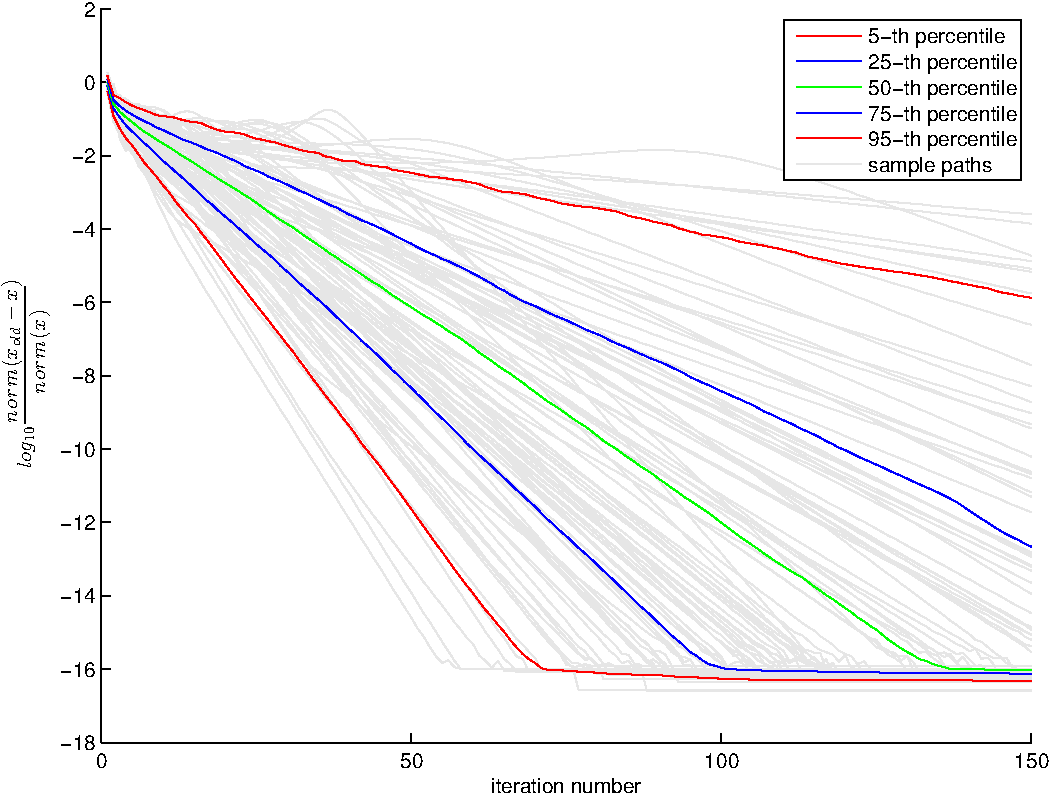
\includegraphics[width=\textwidth]{figures/convergenceBoxPlotDifferentA.pdf}
    \caption[Convergence rates: varying problem instances]{Convergence plot ($1,000$ random matrices $A$, one random $x_0$ per problem instance).}
    \label{fig:qcqpConvVar}
\end{figure}

\begin{figure}[htbp]
    \centering
    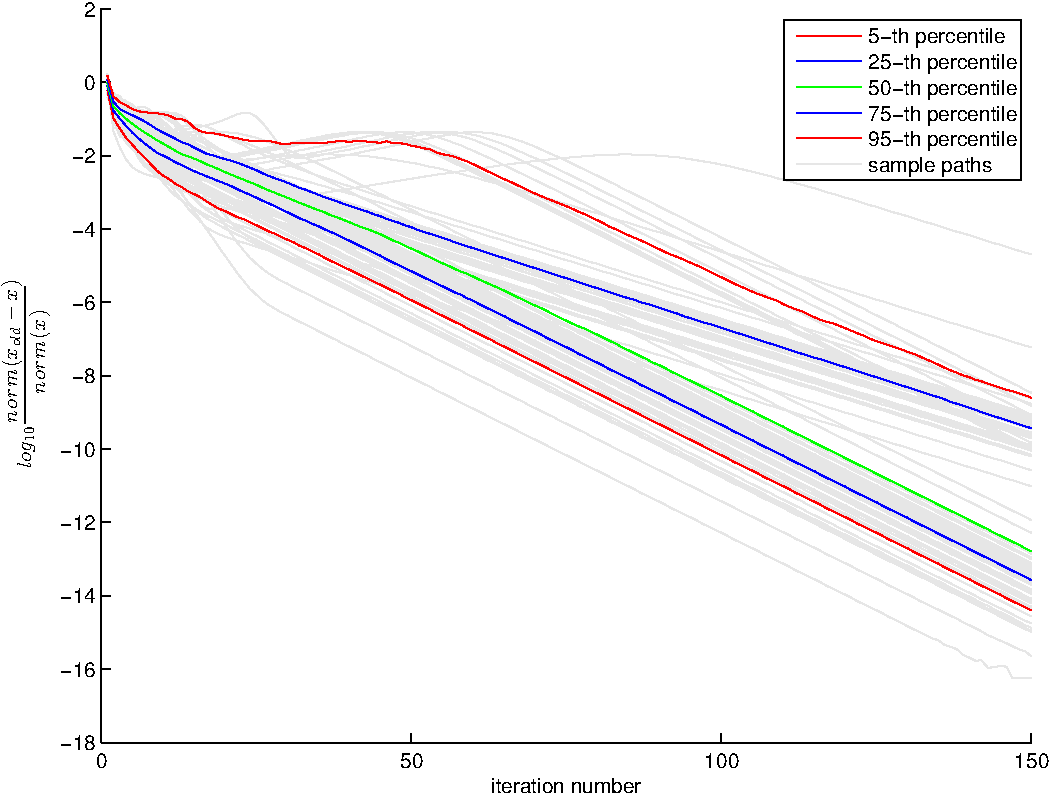
\includegraphics[width=\textwidth]{figures/convergenceBoxPlotFixedA.pdf}
    \caption[Convergence rates: varying initial conditions]{Convergence plot (single random $A$, $1,000$ random initial vectors $x_0$).}
    \label{fig:qcqpConvFix}
\end{figure}

\subsection{SDP and Horst Solutions on Synthetic Problems}\label{chap:experiments:horst}

We also explored how the number of views and the dimensionality of
the problems relates to the difficulty of finding globally optimal
solutions, for all aforementioned methods of generating random problem
instances.
 For each sampling scenario and each choice of $m$ and $n_i$, we generated $100$
experiments, and computed $1,000$ solutions based on Algorithm
\ref{algorithm:horst}, the SDP solution (and respective
global bounds), and examined the frequencies of the following
events:
\begin{itemize}
\item a \textbf{relaxation gap} candidate detected (Tables
\ref{tb:rg}, \ref{tb:rs}, \ref{tb:r1d} (a))
\item \textbf{local convergence} detected (Tables \ref{tb:rg}, \ref{tb:rs},
\ref{tb:r1d} (b))
\item when a local solution is worse
than the SDP-based \textbf{lower bound} (Tables \ref{tb:rg},
\ref{tb:rs}, \ref{tb:r1d} (c)).
\end{itemize}
The possibility of a relaxation gap is
detected when the best local solution is lower than $1\%$ of the
SDP bound. In this case, the event indicates only the possibility
of relaxation gap -- it might be the case that further local
algorithm restarts would close the gap. Local convergence
is detected when the objective value of two local solutions
differs relatively by at least $10\%$ and absolutely at least by
$0.1$ (both criteria must be satisfied
simultaneously). Finally, the event of a local solution being
below the SDP lower bound means that it is below
$\frac{2}{\pi}$ of the optimal objective value of the SDP
relaxation.

We find that regardless of the generation technique, the lower
SDP bound is useful only when $n_i = 1$ (Table \ref{tb:rg},
\ref{tb:rs}, \ref{tb:r1d} (c)) and the results are similar for
different choices of $m$. There are, however, rare instances (less
than $0.1\%$) where the lower bound is useful for $n_i = 2$ and
even rarer (less than $0.01\%$) for $n_i = 3$.

The chance of local convergence increases as the number of views
$m$ increases which can be consistently observed for all choices
of $n_i$ and sampling strategies. Generating a generic problem where the
local algorithm  converges to a local solution is less
likely as the dimensionality increases
(Tables \ref{tb:rg}, \ref{tb:rs}).

In the case of noisy embeddings of a 1-dimensional correlation structures, the dependence on $n_i$
behaves differently: the local convergence (see Table \ref{tb:r1d_lc}) for the
case $\left(m=5, n_i=3\right)$ is more likely than for the
case $\left(m=5, n_i =2\right)$. This is unexpected as in the general case,
increasing $n_i$ reduces that chance of local convergence,
see Table \ref{tb:rs_lc}, Table \ref{tb:rg_lc}.

The relationship between $m$ and $n_i$ and the possibility of a
relaxation gap behaves similarly as local convergence -
increasing $m$ increases it and increasing $n_i$ decreases it (Table \ref{tb:rg_dg}, Table \ref{tb:rs_dg}),
except in the case of noisy 1-dim correlation structures, where
we observe the same anomaly when $n_i = 2$ (Table \ref{tb:r1d_dg}).

Therefore we have demonstrated that there exist sets of problems with nonzero
measure where the SDP bounds give useful information.

\begin{table}[t]
\caption{Random Gram matrix.}
    \begin{subtable}[t]{.5\textwidth}
        \centering
        \caption{Possible relaxation gap.}
        \begin{tabular}{|l|c|c|c|}
\hline
&\textbf{$n_i$ = 3}&\textbf{$n_i$ = 2}&\textbf{$n_i$ = 1}\\\hline
\textbf{$m$ = 5}&0\%&5\%&17\%\\\hline
\textbf{$m$ = 3}&0\%&0\%&9\%\\\hline
\end{tabular}

        \label{tb:rg_dg}
    \end{subtable}
    ~
    \begin{subtable}[t]{.5\textwidth}
        \centering
        \caption{Local convergence.}
        \begin{tabular}{|l|c|c|c|}
\hline
&\textbf{$n_i$ = 3}&\textbf{$n_i$ = 2}&\textbf{$n_i$ = 1}\\\hline
\textbf{$m$ = 5}&1\%&5\%&48\%\\\hline
\textbf{$m$ = 3}&0\%&1\%&26\%\\\hline
\end{tabular}

        \label{tb:rg_lc}
    \end{subtable}
    ~
    \begin{subtable}[t]{\textwidth}
        \centering
        \caption{Local solution below lower SDP bound.}
        \begin{tabular}{|l|c|c|c|}
\hline
&\textbf{$n_i$ = 3}&\textbf{$n_i$ = 2}&\textbf{$n_i$ = 1}\\\hline
\textbf{$m$ = 5}&0\%&0\%&14\%\\\hline
\textbf{$m$ = 3}&0\%&0\%&12\%\\\hline
\end{tabular}

        \label{tb:rg_lb}
    \end{subtable}
  \label{tb:rg}
\end{table}

\begin{table}[t]
  \caption{Random spectrum sampling.}
    \begin{subtable}[t]{.5\textwidth}
        \centering
        \caption{Possible relaxation gap.}
        \begin{tabular}{|l|c|c|c|}
\hline
&\textbf{$n_i$ = 3}&\textbf{$n_i$ = 2}&\textbf{$n_i$ = 1}\\\hline
\textbf{$m$ = 5}&0\%&5\%&36\%\\\hline
\textbf{$m$ = 3}&0\%&1\%&20\%\\\hline
\end{tabular}

        \label{tb:rs_dg}
    \end{subtable}
    ~
    \begin{subtable}[t]{.5\textwidth}
        \centering
        \caption{Local convergence.}
        \begin{tabular}{|l|c|c|c|}
\hline
&\textbf{$n_i$ = 3}&\textbf{$n_i$ = 2}&\textbf{$n_i$ = 1}\\\hline
\textbf{$m$ = 5}&1\%&3\%&50\%\\\hline
\textbf{$m$ = 3}&0\%&0\%&31\%\\\hline
\end{tabular}

        \label{tb:rs_lc}
    \end{subtable}
    ~
    \begin{subtable}[t]{\textwidth}
        \centering
        \caption{Local solution below lower SDP bound.}
        \begin{tabular}{|l|c|c|c|}
\hline
&\textbf{$n_i$ = 3}&\textbf{$n_i$ = 2}&\textbf{$n_i$ = 1}\\\hline
\textbf{$m$ = 5}&0\%&0\%&15\%\\\hline
\textbf{$m$ = 3}&0\%&0\%&16\%\\\hline
\end{tabular}

        \label{tb:rs_lb}
    \end{subtable}
  \label{tb:rs}
\end{table}

\begin{table}[t]
  \caption{Random 1-dim structure sampling.}
    \begin{subtable}[t]{.5\textwidth}
        \centering
        \caption{Possible relaxation gap.}
        \begin{tabular}{|l|c|c|c|}
\hline
&\textbf{$n_i$ = 3}&\textbf{$n_i$ = 2}&\textbf{$n_i$ = 1}\\\hline
\textbf{$m$ = 5}&24\%&16\%&23\%\\\hline
\textbf{$m$ = 3}&7\%&4\%&7\%\\\hline
\end{tabular}

        \label{tb:r1d_dg}
    \end{subtable}
    ~
    \begin{subtable}[t]{.5\textwidth}
        \centering
        \caption{Local convergence.}
        \begin{tabular}{|l|c|c|c|}
\hline
&\textbf{$n_i$ = 3}&\textbf{$n_i$ = 2}&\textbf{$n_i$ = 1}\\\hline
\textbf{$m$ = 5}&9\%&6\%&51\%\\\hline
\textbf{$m$ = 3}&0\%&0\%&31\%\\\hline
\end{tabular}

        \label{tb:r1d_lc}
    \end{subtable}
    ~
    \begin{subtable}[t]{\textwidth}
        \centering
        \caption{Local solution below lower SDP bound.}
        \begin{tabular}{|l|c|c|c|}
\hline
&\textbf{$n_i$ = 3}&\textbf{$n_i$ = 2}&\textbf{$n_i$ = 1}\\\hline
\textbf{$m$ = 5}&0\%&0\%&13\%\\\hline
\textbf{$m$ = 3}&0\%&0\%&15\%\\\hline
\end{tabular}

        \label{tb:r1d_lb}
    \end{subtable}
  \label{tb:r1d}
\end{table}

\section{Experiments on EuroParl Corpus}\label{subsec:documents}

Applications of canonical correlation analysis on collections of
documents include: dimensionality reduction, cross-lingual document retrieval and classification~
\cite{mrpqr}~and~\cite{ccatextdva}, multilingual topic extraction~\cite{mcca} and news bias detection~\cite{ccanewsbias}.
In this section, we explore the behavior of
Algorithm~\ref{algorithm:horst} with respect to the global
bounds on real data, computed based on Algorithm~\ref{algorithm:rpgen},
introduced in Section~\ref{chap:relaxations:practical}.
We start by describing the data and then describe a method to
reduce the dimensionality of the data in order to apply the SDP
bounds.

\subsection{Dataset and preprocessing}
The experiments were conducted on a subset of EuroParl, Release v3,
\cite{europarl}, a multilingual parallel corpus, where our subset
includes Danish, German, English, Spanish, Italian, Dutch,
Portuguese and Swedish. We first removed all documents
which had one translation or more missing. Documents (each
document is a day of sessions of the parliament) were then
arranged alphabetically and split into smaller documents, such that
each speaker instance represented a separate document.
Therefore, we ended up with $12,000$ documents per
language. These roughly correspond to all speeches between 2/25/1999
and 3/25/1999. We then computed the bag of words (vector space)
\cite{Salton88term-weightingapproaches} model for each language,
keeping unigrams, bigrams and trigrams that occurred
more than thirty times. For example: ``Mr'', ``President'' and
``Mr President'' all occurred more than thirty times in the
English part of the corpus and they each represent a dimension in
the vector space.

This resulted in feature spaces with
dimensionality ranging from $50,000$ (English) to $150,000$
(German). Finally, we computed the TF-IDF weighting and normalized
every document for each language. Therefore, we obtained
corpus matrices $X^{(i)}$ for each language, where each
matrix has $12,000$ columns and the columns are aligned
($X^{(i)}\left(:,\ell\right)$ and $X^{(j)}\left(:,\ell\right)$ correspond to
translations of the same text).

\subsection{Local Versus Global Approaches}

We now experimentally address two questions: does the random projection
based approach introduced in Section~\ref{chap:relaxations:practical} enable us to
find \emph{stable patterns} and how informative the SDP
bounds are. Stable patterns are represented by highly correlated directions
in both the training and test sets that were not a part of the parameter
estimation procedure.

The experiments were conducted on the set of five EuroParl
languages: English, Spanish, German, Italian and Dutch. We set
$k = 10$ which corresponds to $n_i = 50$ dimensions per view, so
the QCQP matrix will be of size $250 \times 250$. We randomly
selected $5000$ training documents and $1,000$ test documents.  For
a range of random projection regularization parameters $\gamma$,
we computed the mappings $P_i$ based on the train set, as defined in
Equation~\ref{eq:rp_projectors}. We then used the matrices $P_i$ to
reduce the dimensionality of the training and test sets. Then, for
a range of QCQP regularization parameters $\kappa$, we set up the
QCQP problem, computed $1,000$ local solutions (by Horst
algorithm) and solved the SDP relaxation. The whole procedure was
repeated $10$ times.

For each $(\gamma, \kappa)$ pair, we measured the sum of
correlations on the test and train sets. Table
\ref{tb:textTrainTestSumcor} shows the sums of correlations
averaged over $10$ experimental trials. The maximal possible sum
of correlations for five datasets is $\binom{5}{2} = 10$.
We observed that regularizing the whole optimization problem is
not as vital as regularizing the construction of random
projection vectors. This is intuitive, since finding the
random projection vectors involves a regression in a high
dimensional space, a harder estimation problem as opposed to
solving a lower dimensional QCQP.
The choice of $\gamma = 0.1$ lead to perfectly correlated
solutions on the training set for all $\kappa$ values. This turned out to
be over-fitted when we evaluated the sum of correlations on the
test set. Perfect correlations on the training set were not reproduced on
the test set (the sum of correlations ranges between $5.8$ and $7.4$).
Note that higher $\kappa$ values improved the
performance on the test set up to a certain level below
$7.5$. As we increased $\gamma$ to $0.5$, we saw a reduction in
overfitting and with $\gamma = 0.9$  stable patterns were observed.

We conclude that using appropriate regularization parameters,
we can reduce the dimensionality of the
original QCQP problem and still find stable
solutions.

The reduced dimensionality of the problem then enabled an investigation of
the behavior of the SDP relaxation. For the SDP bounds, we observed behavior that was
similar to the high-dimensional synthetic (generic) case. That is
we found that the potential relaxation gap was very small and that the SDP and the Horst's algorithm yielded the same
result. For this reason we omit the SDP results from Table \ref{tb:textTrainTestSumcor}.

\begin{table}[t]
  \caption{Train and test sum of correlation.}
    \begin{subtable}[t]{\textwidth}
        \centering
        \caption{Train set sum of correlations.}
        \begin{tabular}{|l|c|c|c|c|}
\hline
&\textbf{$\gamma =$0.1}&\textbf{$\gamma =$0.5}&\textbf{$\gamma =$0.9}&\textbf{$\gamma =$0.99}\\\hline
\textbf{$\kappa =$0.01}&10.0&9.8&9.8&9.8\\\hline
\textbf{$\kappa =$0.1}&10.0&9.8&9.8&9.8\\\hline
\textbf{$\kappa =$0.5}&10.0&9.8&9.8&9.8\\\hline
\textbf{$\kappa =$0.9}&10.0&9.8&9.8&9.8\\\hline
\textbf{$\kappa =$0.99}&10.0&9.8&9.7&9.8\\\hline
\end{tabular}

        \label{tb:trainText}
    \end{subtable}
    ~
    \begin{subtable}[t]{\textwidth}
        \centering
        \caption{Test set sum of correlations.}
        \begin{tabular}{|l|c|c|c|c|}
\hline
&\textbf{$\gamma =$0.1}&\textbf{$\gamma =$0.5}&\textbf{$\gamma =$0.9}&\textbf{$\gamma =$0.99}\\\hline
\textbf{$\kappa =$0.01}&5.8&8.6&9.6&9.8\\\hline
\textbf{$\kappa =$0.1}&6.2&8.6&9.6&9.8\\\hline
\textbf{$\kappa =$0.5}&7.0&8.6&9.6&9.8\\\hline
\textbf{$\kappa =$0.9}&7.4&8.8&9.6&9.8\\\hline
\textbf{$\kappa =$0.99}&7.4&8.8&9.6&9.8\\\hline
\end{tabular}

        \label{tb:testText}
    \end{subtable}
  \label{tb:textTrainTestSumcor}
\end{table}

\section{Experiments on the Wikipedia Corpus}\label{sec:evaluation}

We will describe the main dataset for building cross-lingual models, which is
based on Wikipedia, and then present two sets of experiments. The first set of experiments
establishes that the hub based approach can deal with language pairs where little
or no training data is available. The second set of experiments compares the main approaches
that we presented on the task of mate retrieval and the task of event linking. In the mate retrieval task we are given a test set of document pairs, where each pair consists of a document and its translation. Given a query document from the test set, the goal is to retrieve its translation in the other language, which is also referred to as its \emph{mate} document. Finally, we examine how different choices of features impact the event linking performance.

\subsection{Wikipedia Comparable Corpus}

The following experiments are based on a large-scale real-world multilingual dataset
extracted from Wikipedia by using inter-language links for alignment.
Wikipedia is a large source of multilingual data that is especially important for the languages for which no
translation tools, multilingual dictionaries (e.g. Eurovoc~\cite{eurovoc}), or strongly
aligned multilingual corpora (e.g. Europarl~\cite{europarl}) are available. Documents
in different languages are related with so-called \emph{inter-language} links that
can be found on the left of the Wikipedia page. The Wikipedia is constantly growing.
At the time of writing the thesis there were twelve Wikipedias with more than one million articles, $52$ with more
than one hundred thousand articles, $129$ with more than ten thousand articles, and $236$
with more than one thousand articles.

We now present some details on how the dataset was processed to obtain the cross-lingual aligned corpus.
Each Wikipedia page is embedded in the page tag. First, we ignored all the pages whose titles started with a Wikipedia namespace
(which includes categories and discussion pages) and all redirection pages (but we stored the redirect link because inter-language
links can point to redirection links also). We removed the markup of all the pages that we processed.

We constructed the inter-language link matrix using the previously stored redirection links and inter-language links.
Inter-language links that pointed to the redirection links were replaced with the redirection target links. Since linking
is not enforced to be consistent, we obtained a matrix $M$ that was not symmetric. The existence of the inter-language link in
one way (i.e., English to German) does not guarantee that there is an inter-language link in the reverse direction (German to English).
To correct this we symmetrized the matrix $M$ by computing $M+M^T$ and thus obtained an undirected graph. In the rare case that
after symmetrization we had multiple links pointing from a document, we kept the first link. Our experiments were based on
Wikipedia dumps available in 2013.

\subsection{Experiments With Missing Alignment Data}\label{experiments:hubcca}

In this subsection, we will present the empirical performance of hub CCA approach.
We will demonstrate that this approach can be successfully applied even in the case of
fully missing alignment information.
To this purpose, we selected a subset of Wikipedia languages containing three major languages,
English (4,212k articles)--\emph{en} (hub language), Spanish (9,686k articles)--\emph{es},
Russian (9,662k articles)--\emph{ru}, and five minority (in terms of Wikipedia sizes) languages,
Slovenian (136k articles)--\emph{sl}, Piedmontese (59k articles)--\emph{pms},
Waray-Waray (112k articles)--\emph{war} (all with about 2 million native speakers),
Creole (54k articles)--\emph{ht} (8 million native speakers), and Hindi
(97k articles)--\emph{hi} (180 million native speakers). For preprocessing, we removed the documents that contained
less than 20 different words (which are referred to as stubs\footnote{Such documents are typically of low value as a linguistic resource.
Examples include the titles of the columns in the table, remains of the parsing process,
or Wikipedia articles with very little or no information contained in one or two sentences.}) and removed words that occurred in
less than 50 documents as well as the top 100 most frequent words (in each language separately). We represented the documents as
normalized TFIDF~\cite{Salton88term-weightingapproaches} weighted vectors. The IDF scores were computed for each language based
on its aligned documents with the English Wikipedia. The English language IDF scores were computed based on all English documents
for which aligned Spanish documents existed.

The evaluation is based on splitting the data into training and test sets.
We selected the test set documents as all multilingual documents with at least one nonempty alignment
from the list: (\emph{hi}, \emph{ht}), (\emph{hi}, \emph{pms}), (\emph{war}, \emph{ht}), (\emph{war}, \emph{pms}),
the remaining documents are used for training.
The test set is suitable for testing the retrieval between language pairs with possibly empty alignment, since alignments with the hub
language were available.
In Table~\ref{table:train_test}, we display the corresponding sizes of training and test sets for each language pair.

On the training set, we used the two step approach described in Section~\ref{chap:crosslingual:hublang}
to obtain the common document representation as a set of mappings $P_i$.
The test set for each language pair, denoted by $test_{i,j} = \{(x_\ell,y_\ell) | \ell = 1:n(i,j)\} $,
consists of comparable document pairs (linked Wikipedia pages), where $n(i,j)$ is the test set size.
We evaluated the representation by measuring the \emph{mate retrieval} quality on the test sets as follows:
for each $\ell$, we ranked the projected documents $P_j(y_1),\ldots, P_j(y_{n(i,j)})$ according to
their similarity with $P_i(x_\ell)$ and computed the rank of the mate document (aligned document)
$r(\ell) = rank(P_j(y_\ell))$.
The final retrieval score (between -100 and 100) was computed as:
$\frac{100}{n(i,j)} \cdot \sum_{\ell = 1}^{n(i,j)} \left( \frac{n(i,j) - r(\ell)}{n(i,j) -1} -0.5\right)$.
A score that is less than 0 means that the method performed worse than random retrieval and a score of 100
indicates perfect mate retrieval. The mate retrieval results are included in Table~\ref{table:retrieval}.

We observe that the method performs well on all pairs of languages, where at least 50,000 training
documents are available(\emph{en}, \emph{es}, \emph{ru}, \emph{sl}).
We note that taking $k = 500$ or $k = 1,000$ multilingual topics usually results in
similar performance, with some notable exceptions: in the case of (\emph{ht}, \emph{war})
the additional topics result in an increase in performance, as opposed to (\emph{ht}, \emph{pms})
where performance drops, which suggests overfitting. The languages where the method performs
poorly are \emph{ht} and \emph{war}, which can be explained by the quality of data
(see Table~\ref{table:rank} and explanation that follows). In case of \emph{pms}, we demonstrate
that solid performance can be achieved for language pairs (\emph{pms}, \emph{sl})
and (\emph{pms}, \emph{hi}), where only 2,000 training documents are shared between
\emph{pms} and \emph{sl} and no training documents are available between \emph{pms} and \emph{hi}.
Also observe that in the case of (\emph{pms}, \emph{ht}) the method still obtains a
score of 62, even though training set intersection is zero and \emph{ht} data is
corrupted, which we will show in the next paragraph.
{
\renewcommand\tabcolsep{3pt}
\begin{table}[t]
\caption[Training -- test sizes]{Training -- test sizes (in thousands).
The first row represents the size of the training sets used to construct the mappings in low-dimensional language independent space using \emph{en} as a hub. The diagonal elements represent the number of the unique training documents and test documents in each language.
}
\centering
{
\small
\begin{tabular}{c|c|c|c|c|c|c|c|c|}
&	en&	es&	ru&	sl&	hi&	war&	ht&	pms\\\cline{1-9}
en&	671~-~4.6&	463~-~4.3&	369~-~3.2&	50.3~-~2.0&	14.4~-~2.8&	8.58~-~2.4&	 17~-~2.3&	16.6~-~2.7\\
\cline{2-9}
es&	\multicolumn{1}{c|}{}	&	463~-~4.3&	187~-~2.9&	28.2~-~2.0&	8.7~-~2.5&	 6.9~-~2.4&	13.2~-~2&	 13.8~-~2.6\\
\cline{3-9}
ru&	\multicolumn{2}{c|}{}	&	369~-~3.2&	29.6~-~1.9 &	9.2~-~2.7&	2.9~-~1.1&	 3.2~-~2.2&	10.2~-~1.3\\
\cline{4-9}
sl&	\multicolumn{3}{c|}{}	&	50.3~-~2&	3.8~-~1.6&	1.2~-~0.99&	0.95~-~1.2&	 1.8~-~1.0\\
\cline{5-9}
hi&	\multicolumn{4}{c|}{}	&	14.4~-~2.8&	0.58~-~0.8&	0.0~-~2.1&	0.0~-~0.8\\
\cline{6-9}
war&	\multicolumn{5}{c|}{}	&	8.6~-~2.4&	0.04~-~0.5&	0.0~-~2.0\\
\cline{7-9}
ht&	\multicolumn{6}{c|}{}	&	17~-~2.3&	0.0~-~0.4\\
\cline{8-9}
pms&	\multicolumn{7}{c|}{}	&	16.6~-~2.7\\
\cline{9-9}
\end{tabular}
}
\label{table:train_test}
\end{table}
}

{
\renewcommand\tabcolsep{3pt}
\begin{table}[t]
\begin{center}
\caption[Pairwise retrieval]{Pairwise retrieval, 500 topics on the left -- 1,000 topics on the right.}\label{table:retrieval}
\begin{tabular}{|c|c|c|c|c|c|c|c|c|}
\cline{1-9}
&	en&	es&	ru&	sl&	hi&	war&	ht&	pms\\\cline{1-9}
en&	    &	98~-~98&	95~-~97&	97~-~98&	82~-~84&	76~-~74&	53~-~55&	 96~-~97\\
\cline{1-9}
es&	97~-~98&	&	94~-~96&	97~-~98&	85~-~84&	76~-~77&	56~-~57&	96~-~96\\
\cline{1-9}
ru&	96~-~97&	94~-~95&	&	97~-~97&	81~-~82&	73~-~74&	55~-~56&	96~-~96\\
\cline{1-9}
sl&	96~-~97&	95~-~95&	95~-~95&	&	91~-~91&	68~-~68&	59~-~69&	93~-~93\\
\cline{1-9}
hi&	81~-~82&	82~-~81&	80~-~80&	91~-~91&	&	68~-~67&	50~-~55&	87~-~86\\
\cline{1-9}
war&	68~-~63&	71~-~68&	72~-~71&	68~-~68&	66~-~62&	&	28~-~48&	 24~-~21\\
\cline{1-9}
ht&	52~-~58&	63~-~66&	66~-~62&	61~-~71&	44~-~55&	16~-~50&	&	62~-~49\\
\cline{1-9}
pms&	95~-~96&	96~-~96&	94~-~94&	93~-~93&	85~-~85&	23~-~26&	66~-~54&	 \\
\cline{1-9}
\end{tabular}
\end{center}
\end{table}
}

We further inspected the properties of the training sets by roughly estimating the fraction
$\frac{rank(A)}{min\left(rows\left(A\right),~cols\left(A\right)\right)}$ for each English
training matrix and its corresponding aligned matrix of the other language, where $rows(A)$ and $cols(A)$
denote the number of rows and columns respectively. The denominator represents the theoretically
highest possible rank the matrix $A$ could have. Ideally, these two fractions should be
approximately the same - both aligned spaces should have reasonably similar dimensionality.
We display these numbers as pairs in Table~\ref{table:rank}.

\begin{table}[t]
\caption[Dimensionality drift]{Dimensionality drift. Each column corresponds to a pair of aligned corpus matrices between
English and another language. The numbers represent the ratio between the numerical rank and the highest
possible rank. For example, the column $en$ -- $ht$ tells us that for the English-Creole pairwise-aligned
corpus matrix pair, the English counterpart has full rank, but the Creole counterpart is far having full rank.}
\begin{center}
\begin{tabular}{|c|c|c|c|c|c|c|}
\cline{1-7}
en -- es     &   en -- ru     &   en -- sl       &     en -- hi &   en -- war      &      en -- ht &   en -- pms\\
\cline{1-7}
0.81 -- 0.89   &  0.8 -- 0.89  &   0.98 -- 0.96    &    1 -- 1  &  0.74 -- 0.56  &      1 -- 0.22  &   0.89 -- 0.38\\
\cline{1-7}
\end{tabular}
\end{center}
\label{table:rank}
\end{table}

It is clear that in the case of the Creole language only at most $22\%$ documents are unique and suitable
for the training. Though we removed the stub documents, many of the remaining documents are nearly indistinguishable,
as the quality of some smaller Wikipedias is low. This was confirmed for the Creole, Waray-Waray,
and Piedmontese languages by manual inspection. The low quality documents correspond to templates
about the year, person, town, etc. and contain very few unique words.

There is also a problem with the quality of the test data. For example, if we look at the
test pair (\emph{war}, \emph{ht}) only 386/534 Waray-Waray test documents are unique but
on the other side almost all Creole test documents (523/534) are unique. This indicates a poor
alignment which leads to poor performance.


\subsection{Evaluation Of Cross-Lingual Event Linking}
We now turn our attention to the task of cross-lingual event linking and the
evaluation of the novel approach presented in Chapter~\ref{chap:applications}.
In order to determine how accurately we can predict cluster correspondence, we performed two
experiments in a multilingual setting using English, German and Spanish languages for which
we had labelled data to evaluate the linking performance. In the first experiment,
we tested how well the individual approaches for cross-lingual article linking
perform when used for linking the clusters about the same event. In the second
experiment we tested how accurate the prediction model is when trained on different
subsets of learning features. To evaluate the prediction accuracy for a given dataset
we used 10-fold cross validation.

We created a manually labelled dataset in order to evaluate cross-lingual event
linking using two human annotators. The annotators were provided with an interface
listing the articles, their content from and top concepts for a pair of clusters and
their task was to determine if the clusters were in correspondence or not (i.e., discuss same event).
To obtain a pair of clusters $(c_i, c_j)$ to annotate, we first randomly chose a
cluster $c_i$, used Algorithm~\ref{cluster_merge_algo1} to compute a set of potentially
corresponding clusters $C$ and randomly chose a cluster $c_j \in C$. The dataset provided
by the annotators contains 808 examples, of which 402 are cluster pairs in correspondence and
406 are not. Clusters in each learning example are either in English, Spanish or German.
Although Event Registry imports articles in other languages as well, we restricted our
experiments to these three languages. We chose only these three languages since they
have a very large number of articles and clusters per day which makes the cluster linking
problem hard due to large number of possible links.

In Chapter~\ref{chap:background} and Chapter~\ref{chap:crosslingual}, we described the
three main algorithms for identifying similar articles in different languages.
These algorithms were $k$-means, LSI and hub CCA. As a training set, we used common
Wikipedia alignment for all three languages. To test
which of these algorithms performed best, we made the following test. For each of the three
algorithms, we analyzed all articles in Event Registry and for each article computed the
most similar articles in other languages. To test how informative the identified similar
articles are for cluster linking we then trained three classifiers as described in
Section~\ref{algo:features} -- one for each algorithm. Each classifier was allowed
to use as learning features \textbf{only} the cross-lingual article linking features
for which values are determined based on the selected algorithm ($k$-means, LSI and hub CCA).
The results of the trained models are shown in Table~\ref{table:linkingEvalAlgos}. We also show
how the number of topics (the dimensions of the latent space) influences the quality,
except in the case of the $k$-means algorithm, where only the performance on 500 topic
vectors is reported, due to higher computational cost.

We observe that, for the task of cluster linking, LSI and hub CCA perform comparably and both outperform $k$-means.

We also compared the proposed approaches on the task of Wikipedia mate retrieval (the same task as in Section~\ref{experiments:hubcca}).
In our evaluation we used a measure referred to as
the Average Mean Reciprocal Rank (AMRR)~\cite{voorhees1999trec}. Given a collection of $Q$ queries $q_1,\ldots,q_Q$ and
their corresponding mate documents $m_1,\ldots,m_Q$, the Mean Reciprocal Rank (MRR) is expressed as:
$$ MRR = \frac{1}{Q}\sum_{i=1}^Q \frac{1}{rank(i)},$$
where $rank(i)$ refers to the rank position of the mate document $m_i$ with respect to the $i$-th query $q_i$.
The rank is obtained by sorting the similarity scores $\lbrace \textnormal{sim}(q_i,r_j)\rbrace_{j=1}^Q$ in descending order.
Since we are dealing with more than two languages, we averaged the MRR scores over several language pairs and
this aggregate score is referred to as AMRR.

We computed the AMRR performance of the different approaches on the Wikipedia data by holding out $15,000$
aligned test documents and using $300,000$ aligned documents as the training set.

Figure~\ref{pic:AMRR} shows AMRR score as the function of the number of feature vectors.
It is clear that hub CCA outperforms LSI approach and $k$-means lags far behind when testing on Wikipedia data.
The hub CCA approach with $500$ topic vectors manages to perform comparably
to the LSI-based approach with $1,000$ topic vectors, which shows that the CCA
method can improve both model memory footprint as well as similarity computation time.

Furthermore, we inspected how the number of topics influences the accuracy of cluster linking.
As we can see from Table~\ref{table:linkingEvalAlgos} choosing a number of features larger
than $500$ barely affects linking performance, which is in contrast with the fact that additional
topics helped to improve AMMR, see Figure~\ref{pic:AMRR}. Such differences may have arisen
due to different domains of training and testing (Wikipedia pages versus news articles).

We also analyzed how cluster size influences the accuracy of cluster linking. We would
expect that if the tested pair of clusters has a larger number of articles, then the
classifier should be able to more accurately predict whether the clusters should be linked
or not. The reasoning is that the large clusters would provide more document linking information
(more articles mean more links to other similar articles) as well as more accurately aggregated
semantic information. In the case of smaller clusters, the errors of the similarity models have
greater impact which should decrease the performance of the classifier, too. To validate this
hypothesis we have split the learning examples into two datasets -- one containing cluster
pairs where the combined number of articles from both clusters is below 20 and one dataset
where the combined number is 20 or more. The results of the experiment can be seen in
Table~\ref{table:linkingEvalAlgosLargeSmall}. As it can be seen, the results confirm our
expectations: for smaller clusters it is indeed harder to correctly predict if the cluster
pair should be merged or not.

The hub CCA attains higher precision and classification accuracy on the task of linking
small cluster pairs than the other methods, while LSI is slightly better on linking large
cluster pairs. The gain in precision of LSI over hub CCA on linking large clusters is much
smaller than the gain in precision of hub CCA over LSI on linking small clusters. For that
reason we decided to use hub CCA as the similarity computation component in our system.

\begin{figure}
\centering
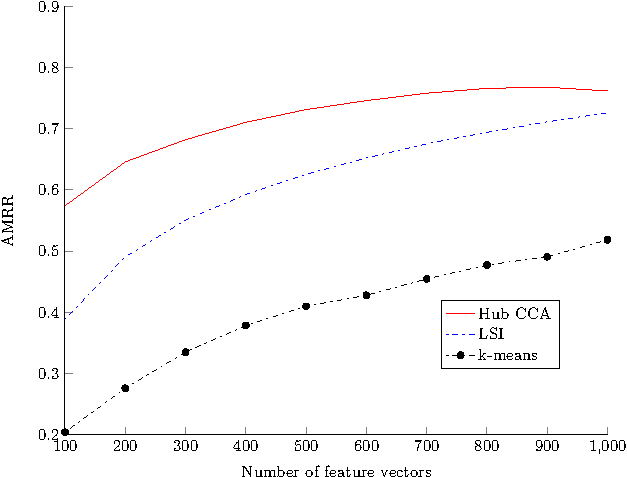
\includegraphics{figures/retrieval.pdf}
\caption{Average of mean reciprocal ranks.}
\label{pic:AMRR}
\end{figure}

\begin{table}[t]
\caption[Accuracy of cluster linking for several cross-lingual similarity models]{Accuracy of cluster linking with 500/800/1,000 topic vectors obtained from
different cross-lingual similarity algorithms. The table shows for each of the algorithms
the obtained classification accuracy, precision and recall. Some results related to $k$-means
are omitted, since the computation took too long and the algorithm's performance was consistently
lower than the other methods considered.}
\begin{center}
\begin{tabular}{|c|c|c|c|c|}
  \hline
  \cline{1-5}
  Models & Accuracy \% & Precision \% & Recall \% & $F_1$ \% \\ \cline{1-5}
  hub CCA  & 78.2/79.6/80.3 & 76.3/78.0/80.5  & 81.6/82.1/79.9 & 78.9/80.0/80.2
  \\ \cline{1-5}
  LSI      & 78.9/78.7/80.6  & 76.8/77.0/78.7 & 83.3/80.6/83.6 & 79.9/78.8/81.1  \\ \cline{1-5}
 $k$-means & 73.9/-/- & 69.5/-/- & 84.6/-/- &  76.3/-/- \\ \cline{1-5}
\end{tabular}
\end{center}
\label{table:linkingEvalAlgos}
\end{table}

\begin{table}[t]
\caption[Accuracy of cluster linking: large vs small clusters]{Accuracy of cluster linking using $500$ topic vectors on two datasets containing large (left number)
and small (right number) clusters. The dataset with small clusters contained the subset of
learning examples in which the combined number of articles from both clusters of the cluster
pair were below 20. The remaining learning examples were put into the dataset of large clusters.}
\begin{center}
\begin{tabular}{|c|c|c|c|c|}
  \hline
  \cline{1-5}
  Models & Accuracy \% & Precision \% & Recall \% & $F_1$ \% \\ \cline{1-5}
  hub CCA  & 81.2 - 77.8 & 80.5 - 74.5 & 91.3 - 57.5 & 85.6 - 64.9 \\ \cline{1-5}
  LSI      & 82.8 - 76.4 & 81.3 - 70.9 & 93.1 - 57.5 & 86.8 - 63.5 \\ \cline{1-5}
 $k$-means & 75.5 - 71.2 & 72.8 - 70.8 & 95.3 - 36.2 & 82.5 - 47.9 \\ \cline{1-5}
\end{tabular}
\end{center}
\label{table:linkingEvalAlgosLargeSmall}
\end{table}

\begin{remark}
Computing hub CCA involves LSI as a preprocessing step which is followed by a low-dimensional
eigen-decomposition, which is negligible when compared to the first step. The computational
complexity of $k$-means is NP-hard, but given a fixed number of iterations, its cost is dominated
by inner product computations (centroids-centroids and dataset-centroids), which is true
for LSI as well when one uses a random-projection based approach~\cite{tropp}.
\end{remark}

In the second experiment, we evaluated how relevant individual groups of features are
to correctly determine cluster correspondence. For this purpose, we computed accuracy using
individual groups of features, as well as using different combinations of groups.
Since hub CCA had the best performance of the three algorithms, we used it to compute
the values of the cross-lingual article linking features. The results of the evaluation
are shown in Table~\ref{table:linkingEval}. We can see that using a single group of features,
the highest prediction accuracy can be achieved using concept-related features.
The classification accuracy in this case is 88.5\%. By additionally including also the
cross-lingual article linking features, the classification accuracy rises slightly
to 89.4\%. Using all three groups of features, the achieved accuracy is 89.2\%.

To test if the accuracy of the predictions is language dependent we have also
performed the evaluations separately on individual language pairs. For this
experiment we have split the annotated learning examples into three datasets,
where each dataset contained only examples for one language pair. When
training the classifier all three groups of features were available. The
results are shown in Table~\ref{table:langPairEval}. We can see that the
performance of cluster linking on the English-German dataset is the highest
in terms of accuracy, precision, recall and $F_1$. The performance on the
English-Spanish dataset is comparable to the performance on the English-German
dataset, where the former achieves higher recall (and slightly higher $F_1$ score),
while the latter achieves higher precision. A possible explanation of these
results is that the higher quantity and quality of English-German language
resources leads to a more accurate cross-lingual article similarity measure
as well as to a more extensive semantic annotation of the articles.

Based on the performed experiments, we can make the following conclusions.
The cross-lingual similarity algorithms provide valuable information that can be
used to identify clusters that describe the same event in different languages.
For the task of cluster linking, the cross-lingual article linking features
are however significantly less informative compared to the concept-related
features that are extracted from the semantic annotations. Nevertheless, the
cross-lingual article similarity features are very important for two reasons.
The first is that they allow us to identify for a given cluster a
limited set of candidate clusters that are potentially in correspondence.
This is a very important feature since it reduces the search space by several
orders of magnitude. The second reason these features are important is
that concept annotations are not available for all articles as the
annotation of news articles is computationally intensive and can only
be done for a subset of collected articles. The prediction accuracies
for individual language pairs are comparable although it seems that
the achievable accuracy correlates with the amount of available language resources.


\begin{table}[t]
\caption[Story linking accuracy for several feature sets]{The accuracy of the classifier for story linking using different sets of learning features.
See Section~\ref{algo:features} for a description of different feature sets that were used in classification: \textbf{Concepts} for concept-related features,
\textbf{Misc} for miscellaneous features and \textbf{Hub CCA} for features based cross-lingual article links using hub CCA.}
\begin{center}
\begin{tabular}{|c|c|c|c|c|}
  \hline
  \cline{1-5}
  Features & Accuracy \% & Precision \% & Recall \% & $F_1$ \%  \\ \cline{1-5}
  Hub CCA            & $78.3 \pm 5.9$ & $78.2 \pm  7.0$ & $78.9 \pm  5.2$ & $78.4 \pm  5.5$ \\ \cline{1-5}
  Concepts           & $88.5 \pm 2.7$ & $88.6 \pm  4.8$ & $88.6 \pm  2.2$ & $88.5 \pm  2.4$ \\ \cline{1-5}
  Misc               & $54.8 \pm 6.7$ & $61.8 \pm 16.5$ & $58.2 \pm 30.2$ & $52.4 \pm 13.0$ \\ \cline{1-5}
  Hub CCA + Concepts & $89.4 \pm 2.5$ & $89.4 \pm  4.6$ & $89.6 \pm  2.4$ & $89.4 \pm  2.3$ \\ \cline{1-5}
  Hub CCA + Misc     & $78.8 \pm 5.0$ & $78.9 \pm  7.1$ & $79.4 \pm  4.6$ & $79.0 \pm  4.5$ \\ \cline{1-5}
  Concepts + Misc    & $88.7 \pm 2.6$ & $88.8 \pm  4.6$ & $88.8 \pm  2.2$ & $88.7 \pm  2.3$ \\ \cline{1-5}
  All                & $89.2 \pm 2.6$ & $88.8 \pm  4.9$ & $90.1 \pm  1.9$ & $89.3 \pm  2.3$ \\ \cline{1-5}
  \hline
\end{tabular}
\end{center}
\label{table:linkingEval}
\end{table}

\begin{table}[t]
\caption[Story linking accuracy for several language pairs]{The accuracy of the classifier for story linking on training data for each language pair separately using all learning features.}
\begin{center}
\begin{tabular}{|c|c|c|c|c|}
  \hline
  \cline{1-5}
  Language pair & Accuracy \% & Precision \% & Recall \% & $F_1$ \% \\ \cline{1-5}
  en, de & $91.8 \pm 5.5$ & $91.7 \pm  6.3$ & $93.7 \pm  6.3$ & $92.5 \pm  5.1$ \\ \cline{1-5}
  en, es & $87.7 \pm 5.4$ & $87.7 \pm  7.4$ & $88.5 \pm  9.8$ & $87.6 \pm  5.9$ \\ \cline{1-5}
  es, de & $88.6 \pm 4.3$ & $89.7 \pm  9.1$ & $84.3 \pm 11.9$ & $85.9 \pm  6.0$ \\ \cline{1-5}
  \hline
\end{tabular}
\end{center}
\label{table:langPairEval}
\end{table}

\subsection{Remarks on the Scalability of the Implementation}

One of the main advantages of our two step approach to cross-lingual cluster linking is that it is highly scalable.
It is fast, very robust to the quality of training data, easily extendable, simple to implement
and has relatively small hardware requirements. The similarity pipeline is the most computationally
intensive part and currently runs on a machine with two Intel Xeon E5-2667 v2, 3.30GHz processors
with 256GB of RAM. This is sufficient to do similarity computation over a large number of
languages if needed. It currently uses Wikipedia as a freely available knowledge base
and experiments show that the similarity pipeline dramatically reduces the search space when linking clusters.

Currently, we compute similarities over $24$ languages with
tags: \emph{eng}, \emph{spa}, \emph{deu}, \emph{zho}, \emph{ita}, \emph{fra}, \emph{rus},
\emph{swe}, \emph{nld}, \emph{tur}, \emph{jpn}, \emph{por}, \emph{ara}, \emph{fin},
\emph{ron}, \emph{kor}, \emph{hrv}, \emph{tam}, \emph{hun}, \emph{slv}, \emph{pol},
\emph{srp}, \emph{cat}, \emph{ukr} but we support any language from the top $100$ Wikipedia languages.
Our data streams come from the service called \emph{Newsfeed} (\url{http://newsfeed.ijs.si/})
which provides 430k unique articles per day.
Our system currently computes 2 million similarities per second, that means that we
compute $16 \cdot 10^{10}$ similarities per day. We
store one day buffer for each language which requires 1.5 GB of memory with documents
stored as 500-dimensional vectors. We note that the time complexity of the similarity
computations scales linearly with dimension of the feature space and does not
depend on the number of languages. For each article, we compute the top $10$ most
similar ones in every other language.

For all linear algebra matrix and vector operations, we use high performance numerical
linear algebra libraries as BLAS, OPENBLAS and Intel MKL, which currently allows
us to process more than one million articles per day.
In our current implementation, we use the variation of the hub approach. Our projector
matrices are of size $500\times 300,000,$ so every projector takes about $1.1$ GB of RAM.
Moreover, we need proxy matrices of size $500\times500$ for every language pair. That
is 0.5 GB for $24$ languages and $9.2$ GB for $100$ languages. Altogether we need
around 135 GB of RAM for the system with 100 languages.
Usage of proxy matrices enables the projection of all input documents in the common
space and handling language pairs with missing or low alignment. That enables us to
do block-wise similarity computations further improving system efficiency. Our code
can therefore be easily parallelized using matrix multiplication rather than performing
more matrix - vector multiplications. This speeds up our code roughly by a factor of 4. In
this way, we obtain some caching gains and ability to use vectorization.
Our system is also easily extendable. Adding a new language requires the computation of
a projector matrix and proxy matrices with all other already available languages.

\subsection{Remarks on the Reproducibility of Experiments}
We have made  both the code and data that were used in the experiments publicly available at \url{https://github.com/rupnikj/jair_paper.git}.
The manually labelled dataset used in the evaluation of event linking is available at in the ``dataset'' subfolder of the github repository. The included archive contains two folders: ``positive'' and ``negative'', where the first folder includes examples of cluster pairs in two languages that represent the same event and the second folder contains pairs of clusters in two languages that do not represent different events. Each example is a JSON file that contains at the top level information about a pair of clusters (including text of the articles) as well as a set of ``meta'' attributes, that correspond to features described in Section \ref{algo:features}.

The ``code'' folder includes MATLAB scripts for building cross-lingual similarity models introduced in Chapter \ref{chap:crosslingual}, which can be used with publicly available Wikipedia corpus to reproduce the cross-lingual similarity evaluation. We have also made available the similarity computation over 100 languages as a service at \url{xling.ijs.si}.

In addition, the Event Registry system (\url{http://eventregistry.org/}) comes with an API, documented at \url{https://github.com/gregorleban/event-registry-python}, that can be used to download events and articles.

